\begin{blocksection}

\question
Even after fixing the undefined behavior of the robots, Avi's team is still losing most of its games! Avi's assistant coach Daniel, in a moment of desperation, suggests an offensive strategy where Player 3 is always on the attack. This is represented by a continuous high output of the register representing Player 3. Draw the input instruction that would make Player 3's output high for all time after 44ps, or state why this is not possible.

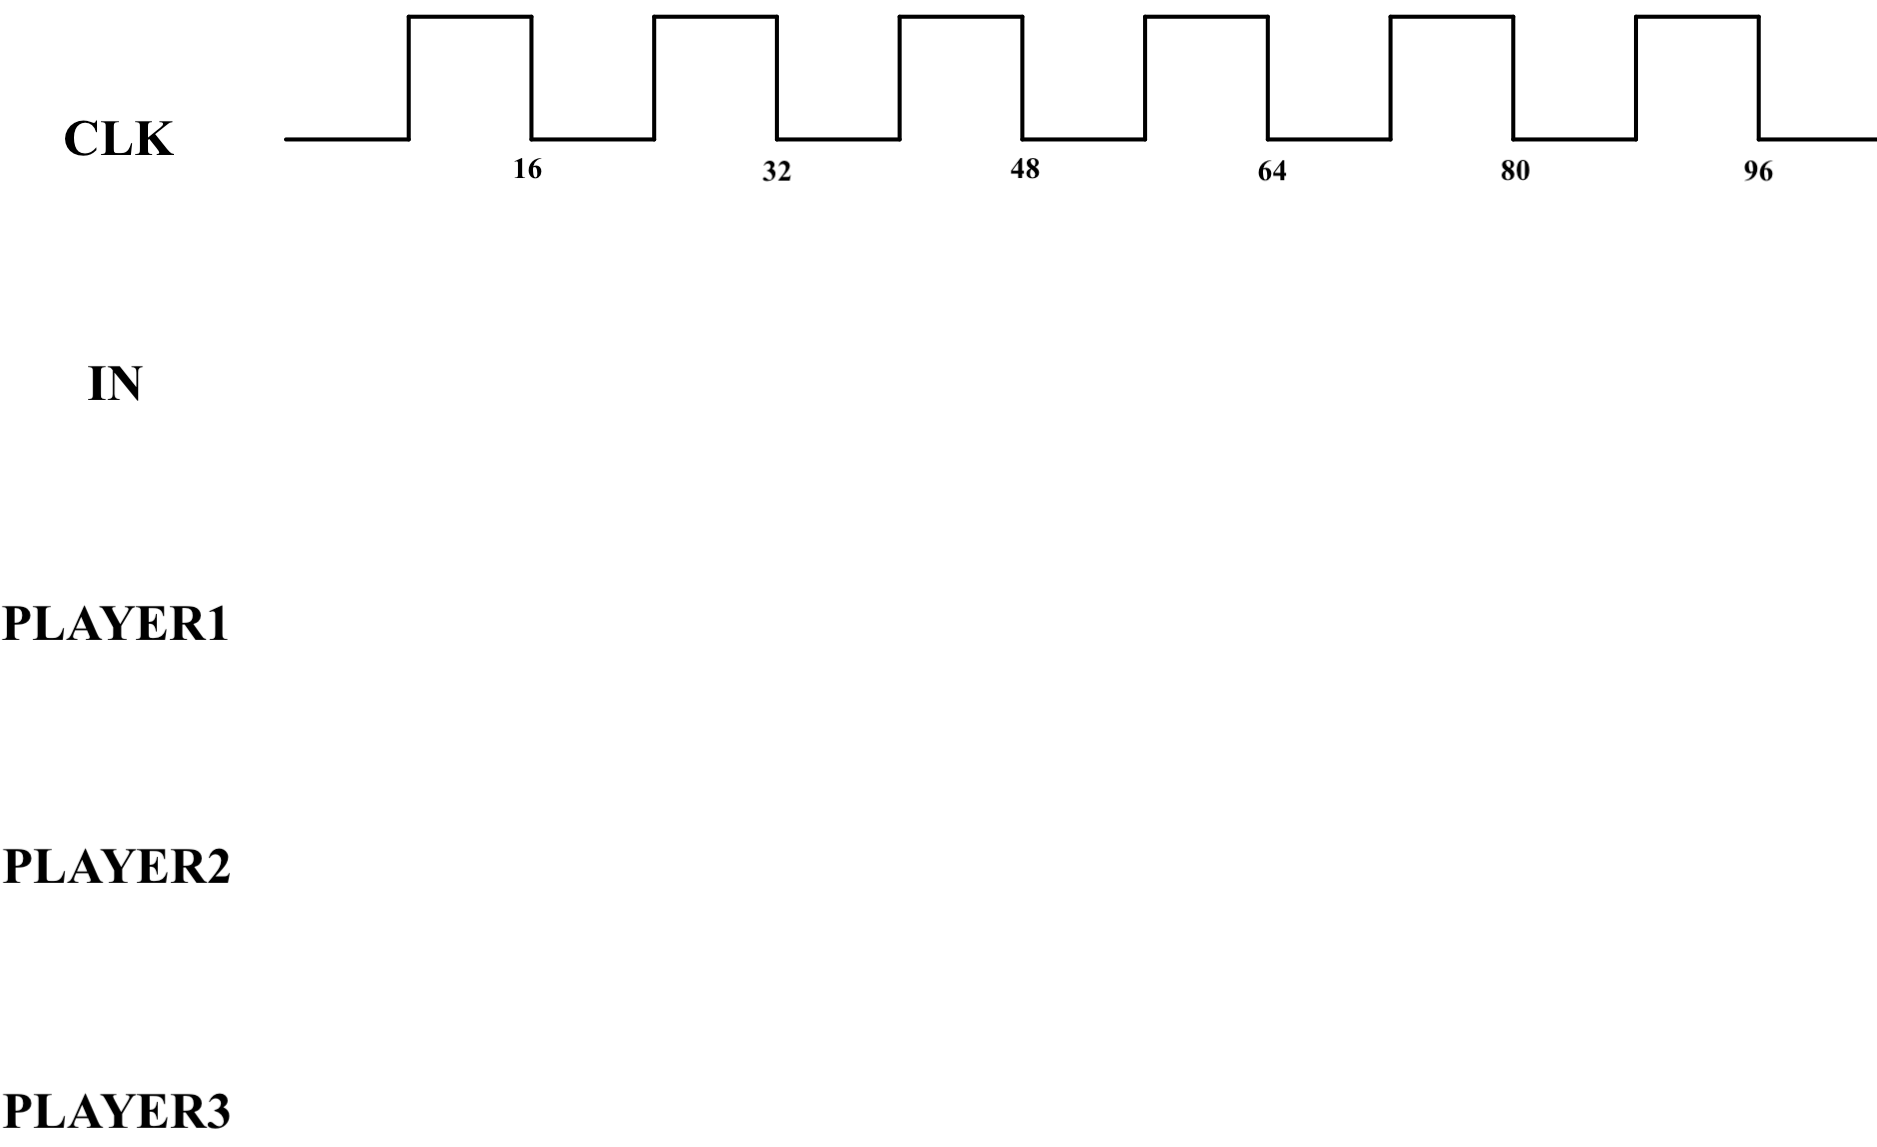
\includegraphics[width=\textwidth]{sds/bball_clock}

\begin{solution}
This is not possible with the circuit given. Both the output of the Player2 register and the input to the Player1 register must be high in order for Player3 register to output high. 
However, by definition, the Player2 output is the opposite of the Player1 output from the clock cycle before. 
Since the input to any register needs to be constant for 8 ps before the rising edge of the clock, the input to the AND gate must be constant for 10 ps before the rising edge of the clock. 
So we can’t flip the input from low to high in time for the register to read, without causing a setup time violation. In fact, we can’t keep the output of Player3’s register high for longer than one clock cycle! Looks like Daniel's strategy can't be implemented
\end{solution}

\end{blocksection}